\documentclass[12pt]{article}

\usepackage{cmap}
\usepackage[T2A]{fontenc}
\usepackage[russian]{babel}
\usepackage[utf8]{inputenc}

\usepackage{algorithm}
\usepackage{algpseudocode}
\usepackage{amsfonts}
\usepackage{amssymb, amsmath, mathrsfs, amsthm}
\usepackage{bbm}
\usepackage{bm}
\usepackage[footnotesize]{caption2}
\usepackage{color}
\usepackage{csvsimple}
\usepackage{fancyvrb}
\usepackage{graphicx}
\usepackage[hidelinks]{hyperref}
\usepackage{indentfirst}
\usepackage{listings}
\usepackage{mathtools}
\usepackage{multirow}
\usepackage{pgfplots}
\pgfplotsset{compat=1.18}

\usepackage{tikz}
\usepackage{wrapfig}
\usepackage{yfonts}

% Параметры страницы
\textheight=24cm
\textwidth=16cm
\oddsidemargin=5mm
\evensidemargin=-5mm
\marginparwidth=36pt
\topmargin=-2cm
\footskip=2.5em
\footnotesep=2ex
\flushbottom
\raggedbottom
\tolerance 3000
% подавить эффект "висячих строк"
\clubpenalty=10000
\widowpenalty=10000
\renewcommand{\baselinestretch}{1.1}
\renewcommand{\baselinestretch}{1.5} %для печати с большим интервалом

% Дополнительные команды для личных обозначений
\DeclareMathOperator*{\argmax}{arg\,max}
\DeclareMathOperator*{\argmin}{arg\,min}

\newcommand{\lt}{\textless}    % знак меньше
\newcommand{\gt}{\textgreater} % знак больше

\newtheorem{definition}{Определение}
\newtheorem{statement}{Утверждение}

% \usepackage{graphicx}
% \usepackage{epstopdf}
% \epstopdfDeclareGraphicsRule{.pdf}{png}{.png}{%
%   wsl convert -density 500 #1 \OutputFile
% }
% \AppendGraphicsExtensions{.pdf}

\begin{document}

\begin{titlepage}
\begin{center}
    Московский государственный университет имени М. В. Ломоносова

    \bigskip
    
\includegraphics[width=50mm]{msu.eps}

    \bigskip
    Факультет Вычислительной Математики и Кибернетики\\
    Кафедра Математических Методов Прогнозирования\\[10mm]

    \textsf{\large\bfseries
        Задание 3.\\[10mm]
        <<Задание 3. Ансамбли алгоритмов. Веб-сервер. Композиции алгоритмов для решения задачи регрессии>>
    }\\[10mm]

    \begin{flushright}
        \parbox{0.5\textwidth}{
        	Выполнилa:\\
        	студентка 3 курса 317 группы \\
        	\emph{Никишкина Евгения Геннадьевна}\\[5mm]
        }
    \end{flushright}

    \vspace{\fill}
    Москва, 2022
\end{center}
\end{titlepage}


\newpage
\renewcommand{\contentsname}{Содержание}
\tableofcontents

\newpage
\begin{section}{Введение}
В статистике и машинном обучении под ансамблем моделей понимают комбинацию нескольких алгоритмов обучения, которые, работая вместе, позволяют построить модель более эффективную и точную, чем любая из моделей, построенная с помощью отдельного алгоритма. Одним из подходов к построению композиций является \emph{бэггинг}, основная идея которого заключается в построении отдельных моделей и усреднению их ответов. \emph{Метод случайных лесов} основан на бэггинге над решающими деревьями. Альтернативный подход к построению композиций является \emph{бустинг}, основанный на последовательном построении моделей, каждая из которых исправляет ошибки предыдущей. Такой подход используется в \emph{градиентном бустинге}.

Данное задание направлено на ознакомление с алгоритмами композиций: случайный лес и градиентный бустинг. Основными этапи являются: создание собственной реализации данных алгоримтов, проведение экспериментов на датасете данных о продажах недвижимости, аналих полученных результов, реализация веб-сервера для взаимодействия с моделью.
\end{section}
\begin{section}{Пояснения к задаче}
Пусть дана конечная $X = (x_i, y_i)$ с вещественными ответами.
Рассмотрим задачу линейной регрессии с метрикой RMSE:
$RMSE = \sqrt{\frac{1}{n}\sum_{i=1}^n(pred_i - y_i)^2}$, где $y_i$ - истинный ответ для $i$-ого объекта, $pred_i$ - предсказание для $i$-ого объекта, $n$ - количество объектов в выборке.
\end{section}
\begin{section}{Предобработка данных}
Эксперименты в ходе задания проводились на датасете данных о продажах недвижимости \emph{House Sales in King County, USA}. Исходные данные содержат 21 признак, включая целевую переменную \emph{price}, которую необходимо отделить в соответствующей столбец целевой переменной. Столбец \emph{date} с данными о дате был разделен на 4 столбца: год, месяц, день месяца и день недели. Также из данных был удален столбец \emph{id}. Пропущенные значения были заполнены с помощью модуля SimpleImputer, используя стратегию заполнения средним значением. 

\begin{figure}[h]
\centering
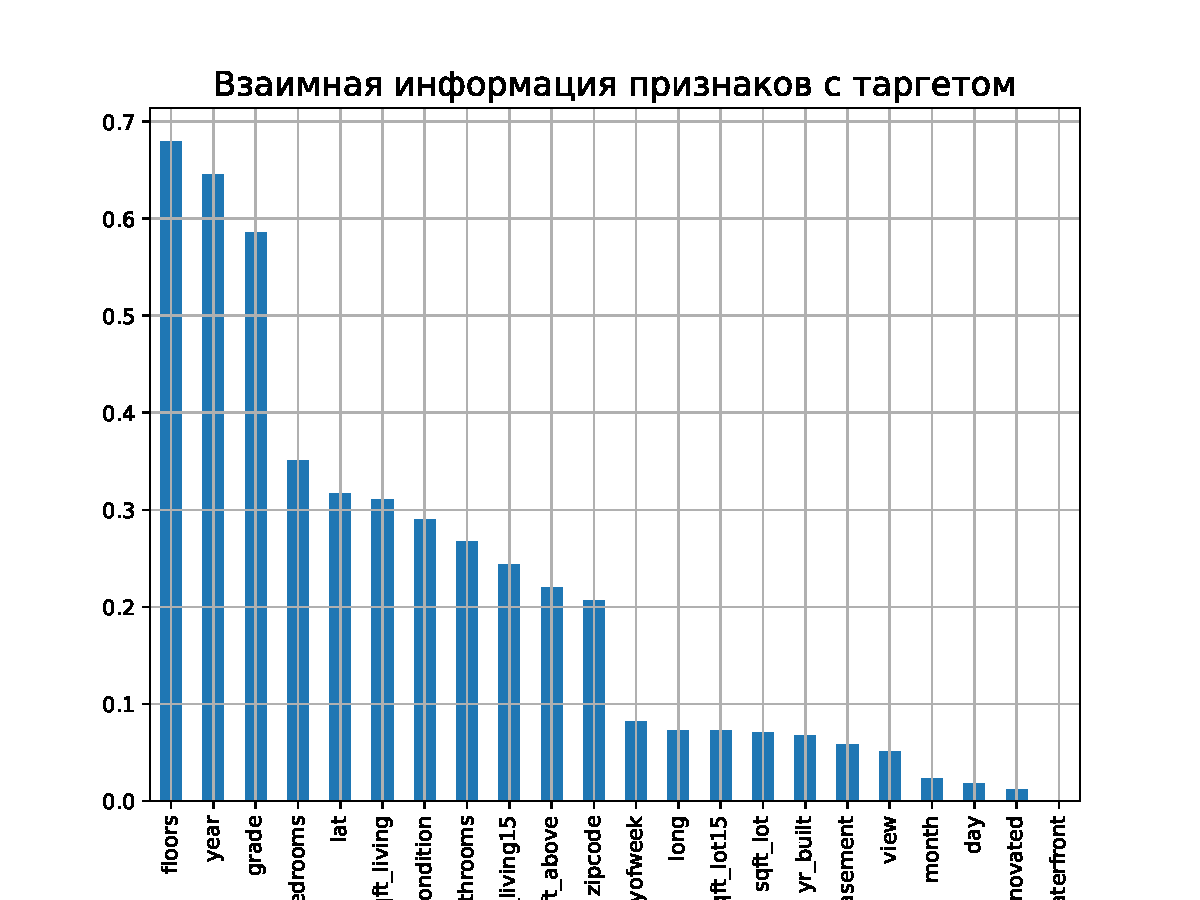
\includegraphics[width=1\linewidth]{1.pdf}
\caption{Взаимная информация признаков с целевой переменной}
\label{fig:mpr}
\end{figure}

Для того чтобы понять, какие признаки оказывают влияние на целевое значение, а какие нет одним из способов может быть расчет корреляции, однако она показывает только линейные зависимости. В отличие от корреляции «взаимная информация» позволяет определить любые виды влияния признаков на целевое значение. Взаимная информация показывает хорошие результаты, если эмпирические плотности $p(x), \; p(y), \; p(x, y)$, полученные по обучающей выборке, хорошо оценивают истинные плотности. Число объектов в обучающей выборке достаточно большое, поэтому есть надежда на хорошую оценку плотностей. Благодаря данной оценке были удалены признаки: день месяца, год ремонта и переменная, отвечающая за наличия вида на набережную. Кажется, довольно странным удаление последнего из этих признаков, ведь, если дом имеет вид на набережную, то его цена должна быть значительно больше чем у дома без такого вида, однако среднее значение, которое принимает данный признак, равно 0.0075, что свидетельствует о том, что большинство домов не имеет вида на набережную, то есть переменная не является информативной.

Среди данных был выделен такой категориальный признак, как почтовый индекс, требующих предобработки. Существует множество методов, позволяющих обрабатывать категориальные признаки. One-hot-кодирование может сильно увеличивать количество признаков в датасете, что сказывается на памяти и времени вычислений, особенно, когда признак имеет большое количество значений. Эту проблему решает такой способ кодирования категориальных признаков как счётчики. Основная идея состоит в том, что нам важны не сами категории, а значения целевой переменной, которые имеют объекты этой категории. Поэтому для кодирования категориального признака был выбран метод Target Encoding со сглаживанием с коэффициентом 1 (по умолчанию). Сглаживание при использовании данного подхода важно, потому что позволяет избежать утечки целевой переменной. В результате предобработки данных размерность признакового пространства стала равна 19. Выборка была разделена на обучающую и тестовую в соотношении 7:3.
\end{section}
\begin{section}{Метод случайных лесов}

В данном эксперименте необходимо было исследовать поведение алгоритма: изучить \emph{RMSE} и его время работы в зависимости от следующих параметров: количество деревьев в ансамбле, размерность подвыборки признаков для одного дерева и максимальная глубина дерева. При исследовании поведения алгоритма в зависимости от числа деревьев в ансамбле параметры, отвечающие за максимальную глубину деревьев и размерность признакового пространства были выбраны по умолчанию, то есть максимальная глубина не ограничена, а размерность признакового пространства $[\frac{n}{3}]$, где $n$ - количество признаков. Для оценки времени работы функций использовалась функция time() из модуля time. 
По результатам экспериментов видно, что RMSE с ростом числа деревьев монотонно уменьшается до точки, в которой достигается оптимум - 883 деревьев для валидационной выборки при гиперпараметрах, установленных по умолчанию. По графику зависимости времени наблюдается линейная зависимость от числа деревьев.


\begin{figure}[h]
\begin{minipage}[h]{0.5\linewidth}
\center{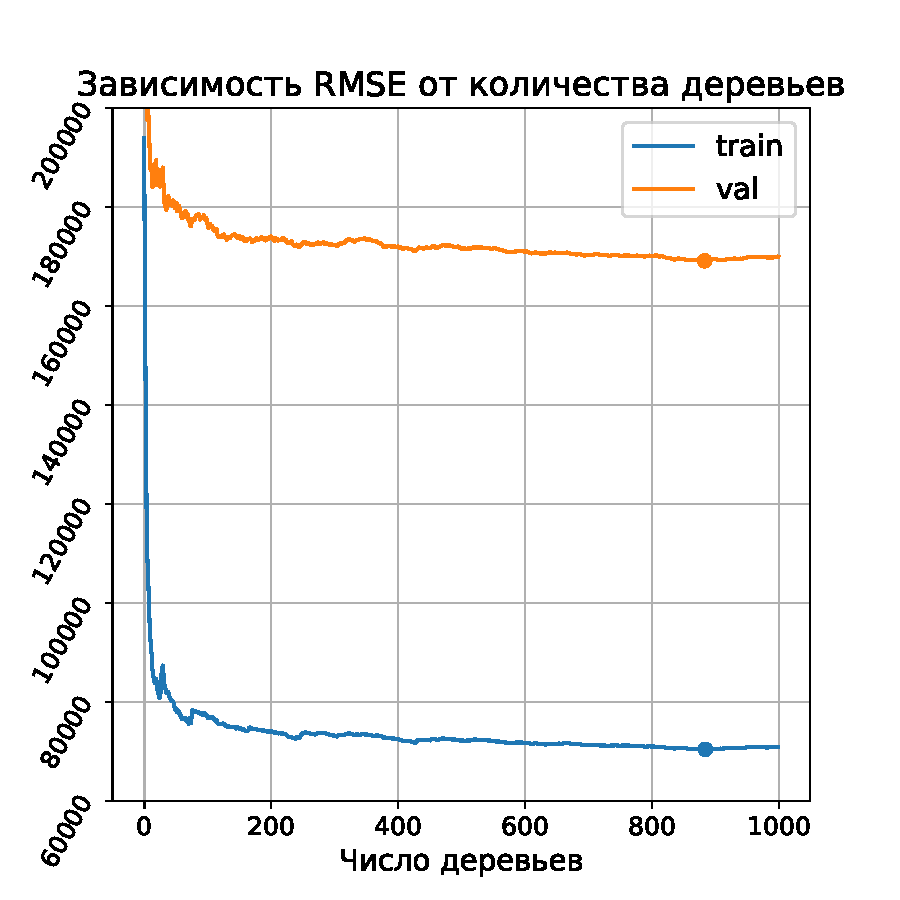
\includegraphics[width=1\linewidth]{2_1.pdf}}
\end{minipage}
\hfill
\begin{minipage}[h]{0.5\linewidth}
\center{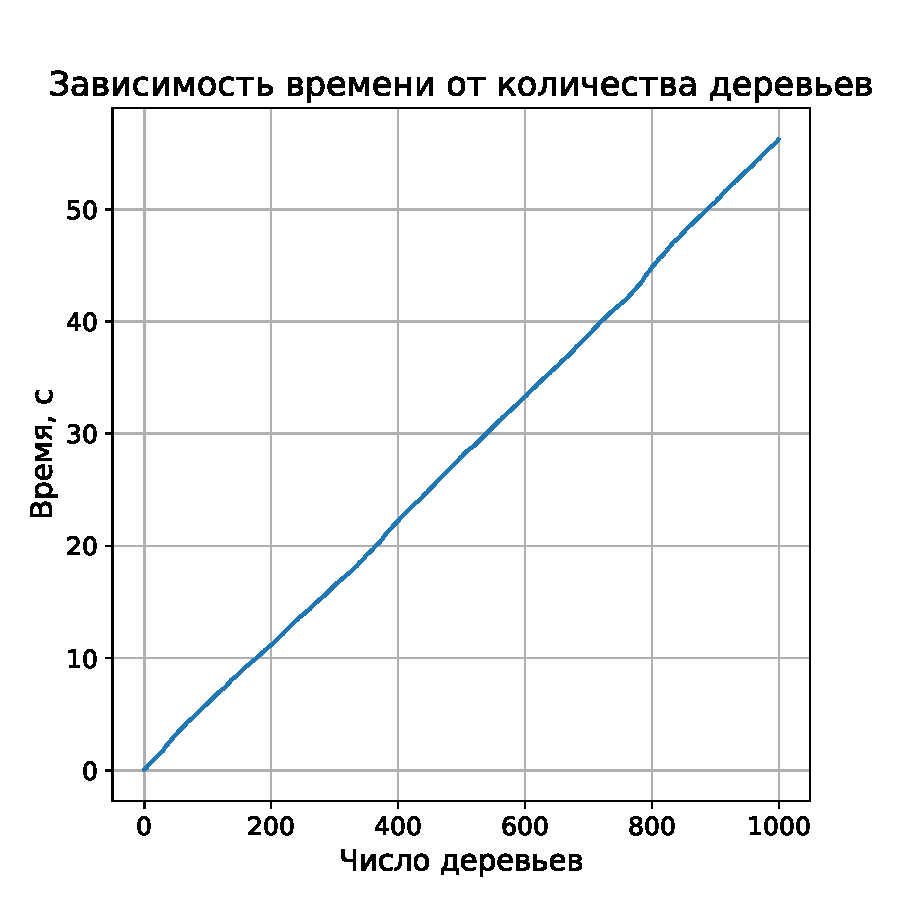
\includegraphics[width=1\linewidth]{2_2.pdf}}
\end{minipage}
\caption{Исследование поведения алгоритма в зависимости от количества деревьев в ансамбле}
\label{ris:image1}
\end{figure} 

При исследовании зависимости от числа признаков параметр максимальной глубины дерева был установлен по умолчанию. По графикам видно, что с увеличением числа признаков ошибка RMSE работы алгоритма уменьшается и минимум на валидационной выборке достигается при использовании всех признаков, то есть 19.

\begin{figure}[h!]
\begin{minipage}[h]{0.5\linewidth}
\center{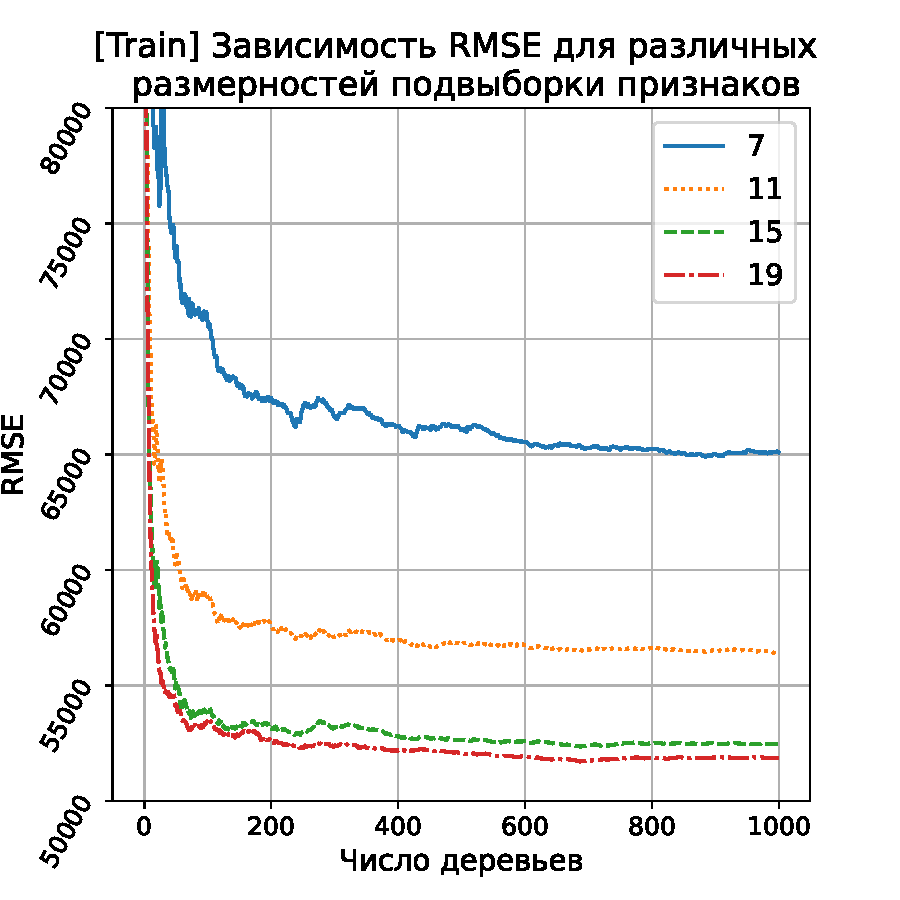
\includegraphics[width=1\linewidth]{2_3.pdf}}
\end{minipage}
\hfill
\begin{minipage}[h]{0.5\linewidth}
\center{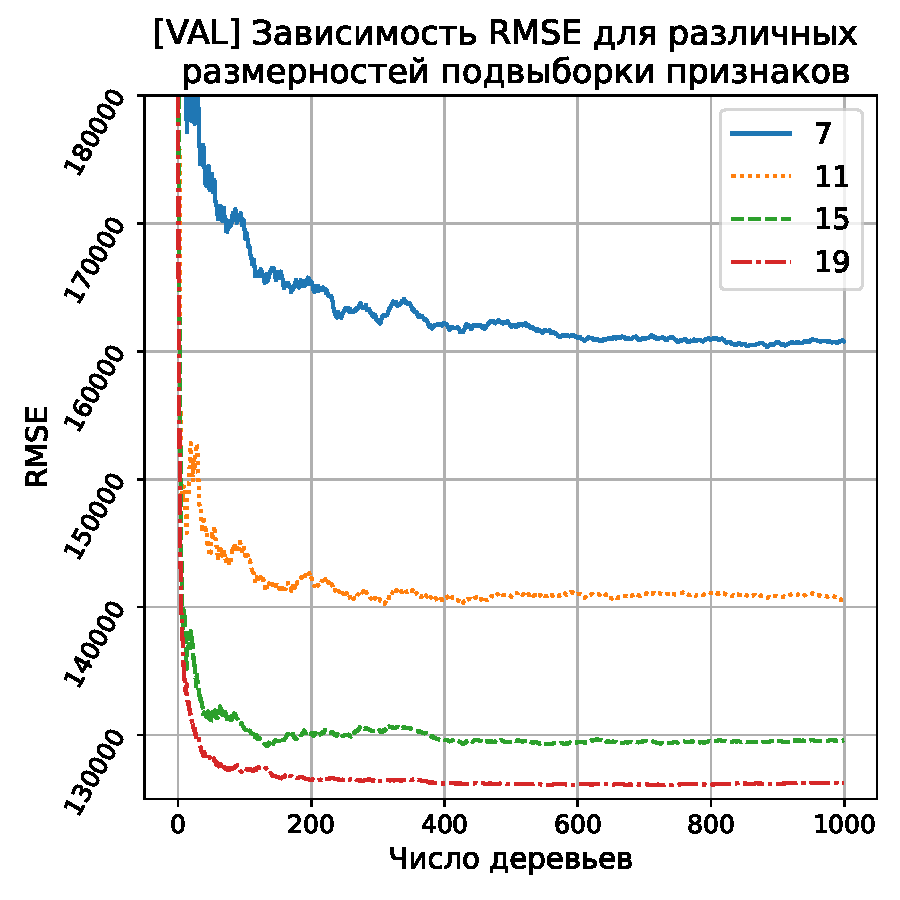
\includegraphics[width=1\linewidth]{2_4.pdf}}
\end{minipage}
\caption{Исследование поведения алгоритма в зависимости от размерности признакового пространства}
\label{ris:image1}
\end{figure}

\newpage
Исследование зависимости от максимальной глубины дерева проводилось с фиксированной размерностью признакового пространства, равной 19. Обычно в данном алгоритме строятся глубокие деревья, что сказывается на времени работы данного метода, однако ограничение на глубину деревьев, способное решить данную проблему, снижает точность. Из графиков видно, что наименьшая ошибка достигается при отсутствии ограничений на максимальную глубину. 

\begin{figure}[h]
\begin{minipage}[h]{0.5\linewidth}
\center{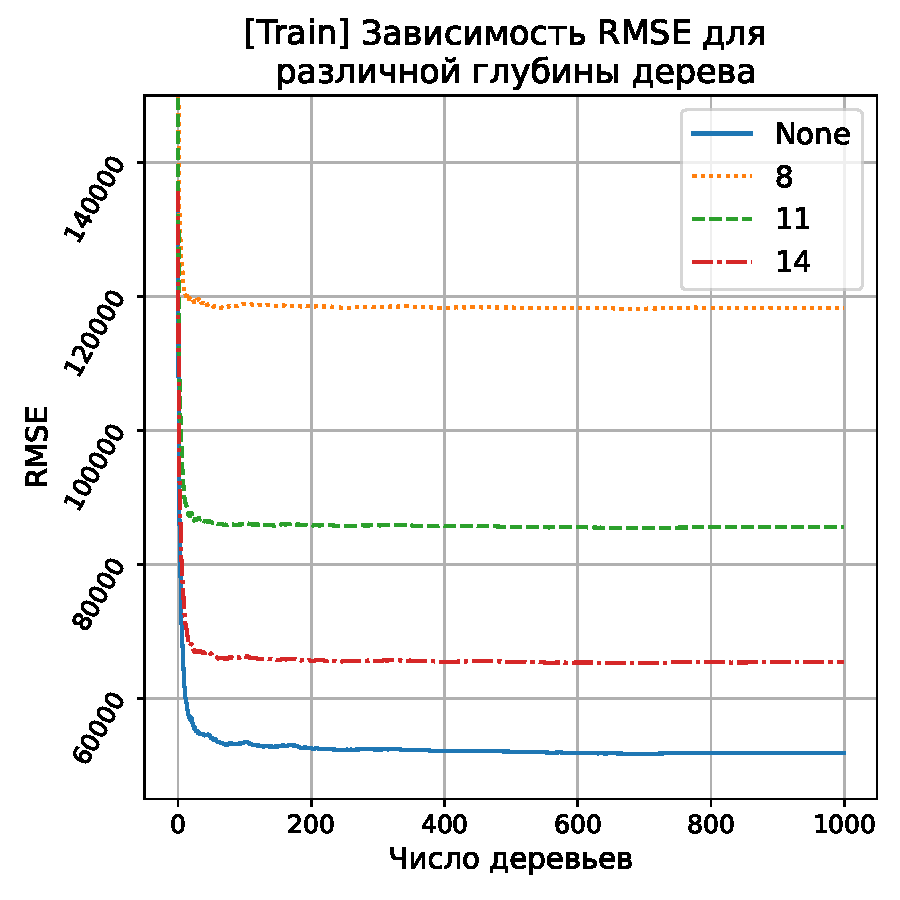
\includegraphics[width=1\linewidth]{2_6.pdf}}
\end{minipage}
\hfill
\begin{minipage}[h]{0.5\linewidth}
\center{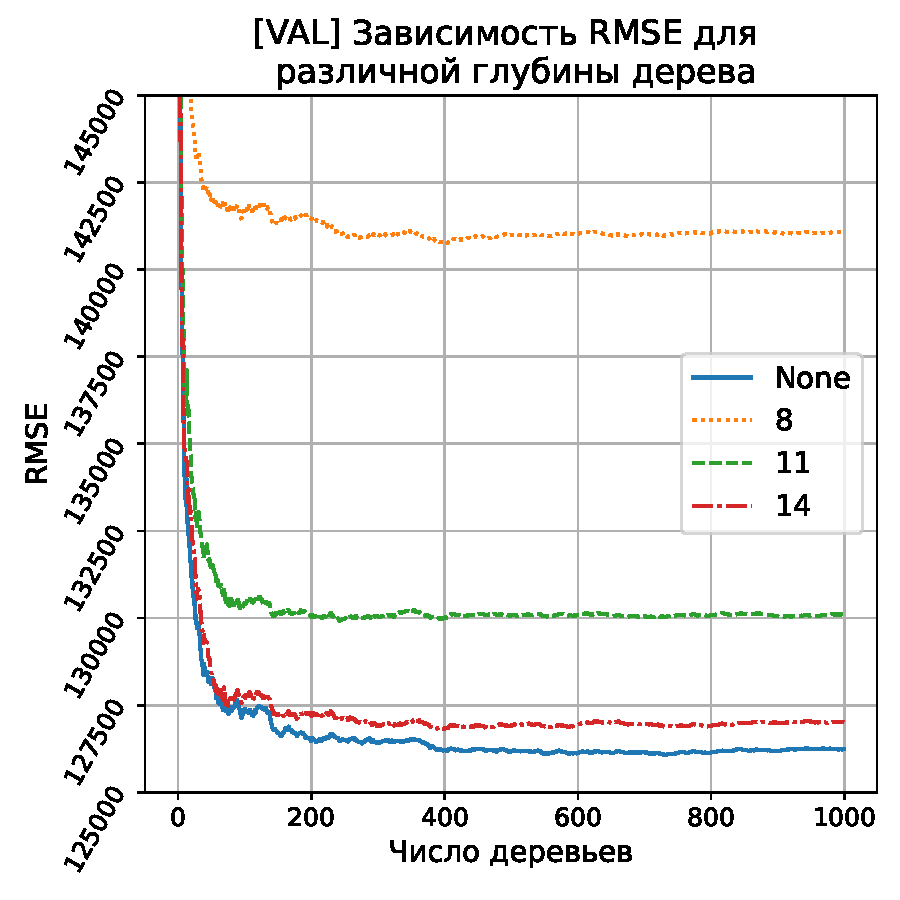
\includegraphics[width=1\linewidth]{2_7.pdf}}
\end{minipage}
\caption{Исследование поведения алгоритма в зависимости от максимальной глубины деревьев}
\label{ris:image1}
\end{figure}



\begin{figure}[h!]
\begin{minipage}[h]{0.5\linewidth}
\center{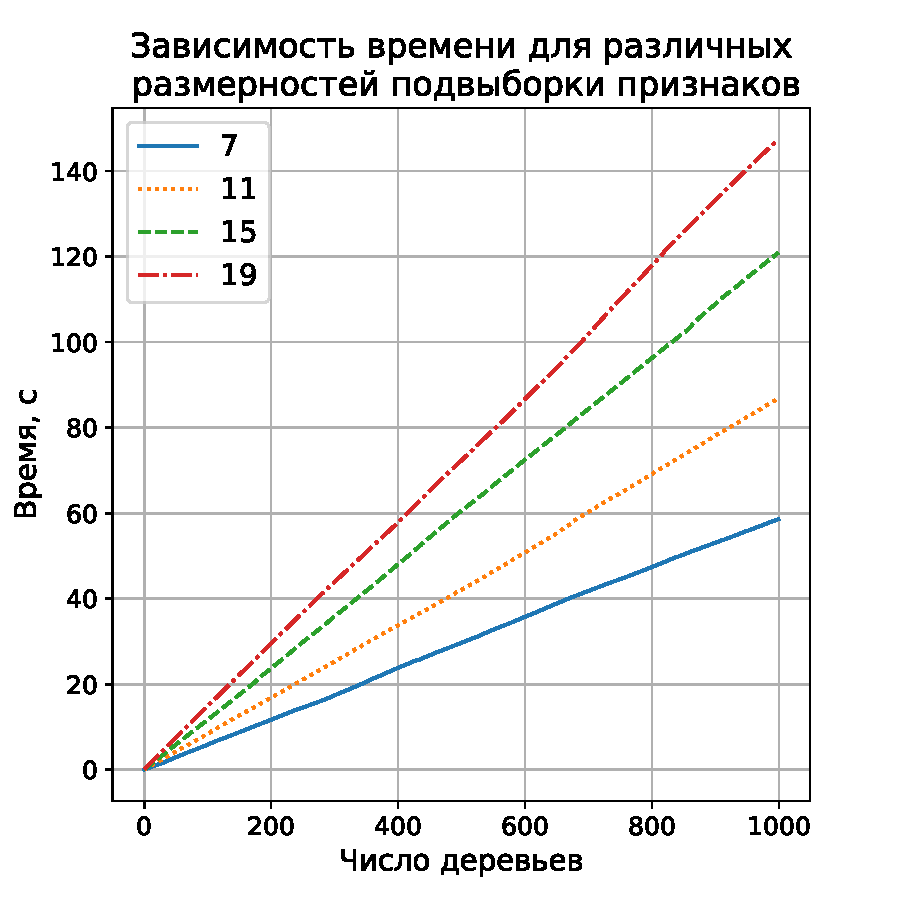
\includegraphics[width=1\linewidth]{2_5.pdf}}
\end{minipage}
\hfill
\begin{minipage}[h]{0.5\linewidth}
\center{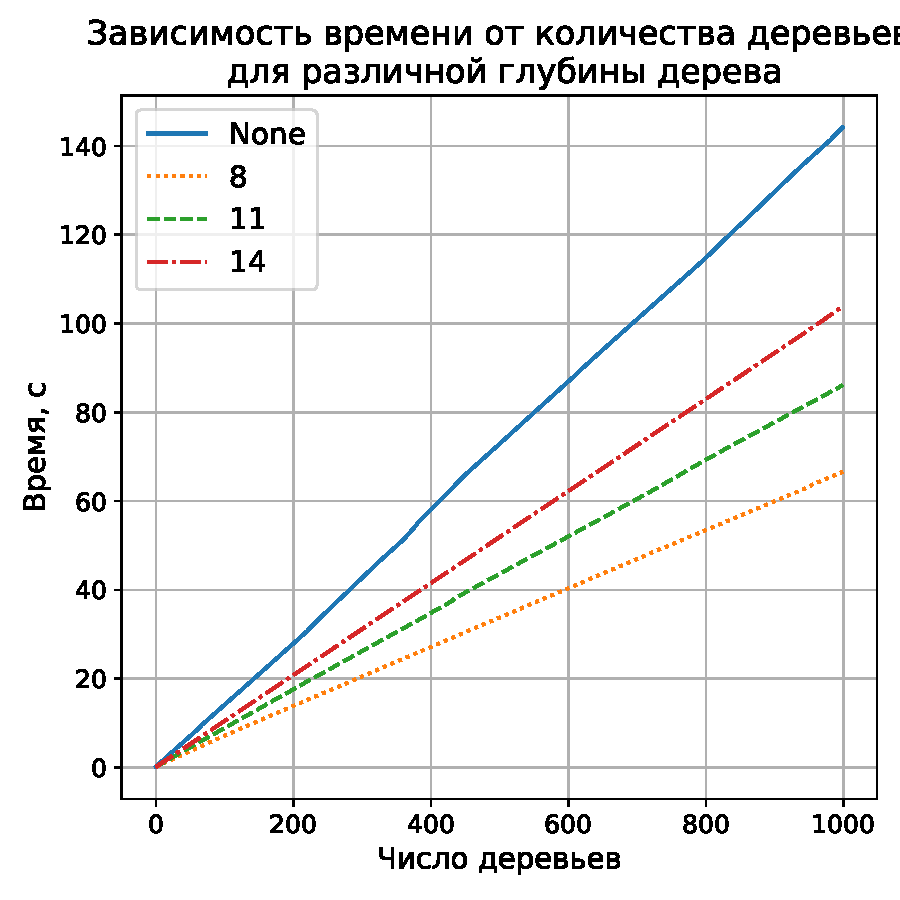
\includegraphics[width=1\linewidth]{2_8.pdf}}
\end{minipage}
\caption{Исследование времени  работы алгоритма в зависимости от параметров}
\label{ris:image1}
\end{figure}

\newpage

Графики, демонстрирующие зависимость времени работы алгоритмов от размерности пространства признаков и максимальной глубины деревьев, показывают, что с ростом глубины дерева время работы алгоритма увеличивается, что наблюдается и в случае увеличения количества признаков в дереве. В каждом из случаев зависимость является линейной, так как при фиксированном числе деревьев расстояния между графиками равны.
\end{section}
\begin{section}{Градиентный бустинг}
В данном эксперименте необходимо было исследовать поведение алгоритма: изучить \emph{RMSE} и его время работы в зависимости от следующих параметров: количество деревьев в ансамбле, размерность подвыборки признаков для одного дерева, максимальная глубина дерева и темп обучения. При исследовании поведения алгоритма в зависимости от числа деревьев в ансамбле параметры, отвечающие за максимальную глубину деревьев (5), размерность признакового пространства и темп обучения (0.1) были выбраны по умолчанию.

\begin{figure}[h!]
\begin{minipage}[h]{0.5\linewidth}
\center{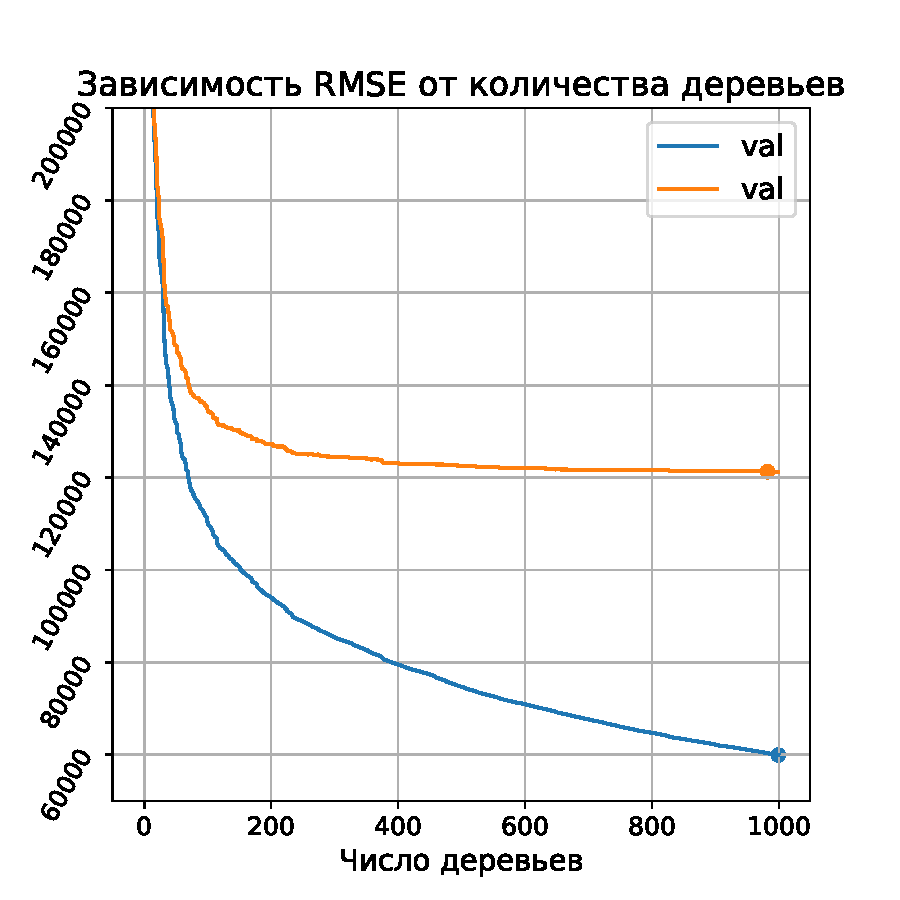
\includegraphics[width=1\linewidth]{3_1.pdf}}
\end{minipage}
\hfill
\begin{minipage}[h]{0.5\linewidth}
\center{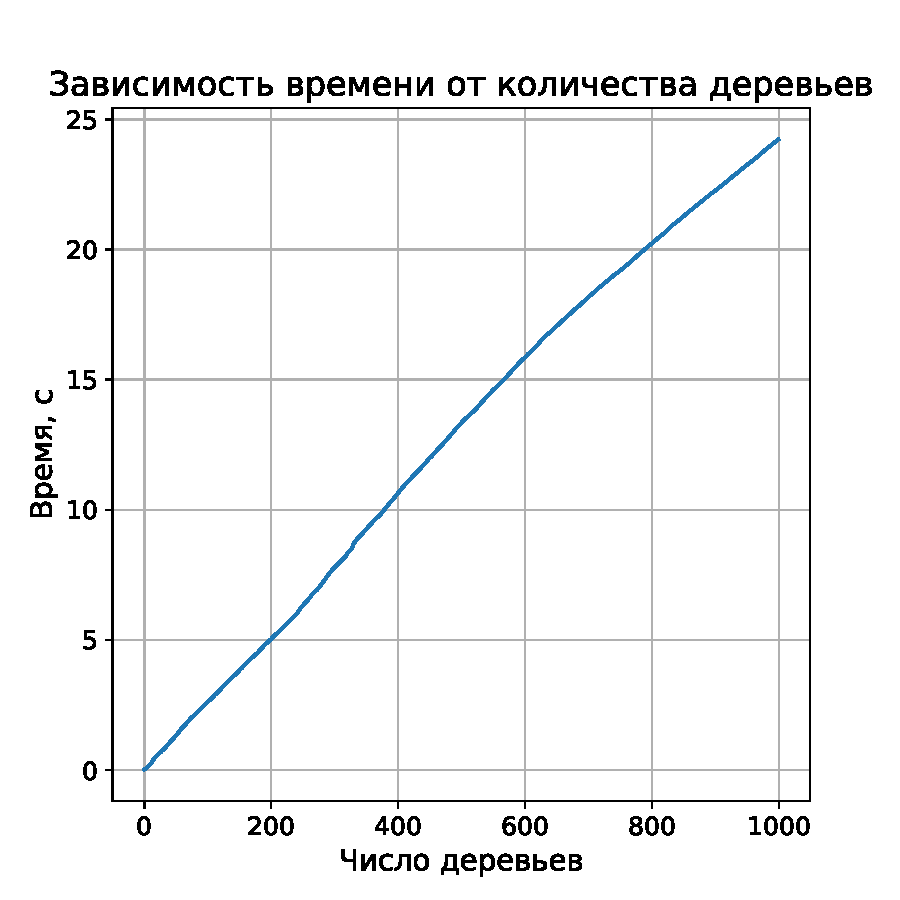
\includegraphics[width=1\linewidth]{3_2.pdf}}
\end{minipage}
\caption{Исследование поведения алгоритма в зависимости от количества деревьев в ансамбле}
\label{ris:image1}
\end{figure}

В ходе обучения случайного леса каждый базовый алгоритм строится независимо от остальных. Бустинг, в свою очередь, воплощает идею последовательного построения линейной комбинации алгоритмов. Каждый последующий базовый алгоритм исправляет ошибки предыдущего. Видно, что графики для данного подхода выглядят более сглаженными, чем в случае метода случайных лесов. По результатам экспериментов видно, что \emph{RMSE} с ростом числа деревьев монотонно уменьшается, оптимальное значение достигается при 982 деревьях. График зависимости времени характеризуется линейной зависимостью от числа деревьев. Отметим, что время работы градиентного бустинга практически в 2 раза меньше времени работы метода случайного леса, это связано с тем, что в градиентном бустинге глубина деревьев меньше. 

\begin{figure}[h!]
\begin{minipage}[h]{0.5\linewidth}
\center{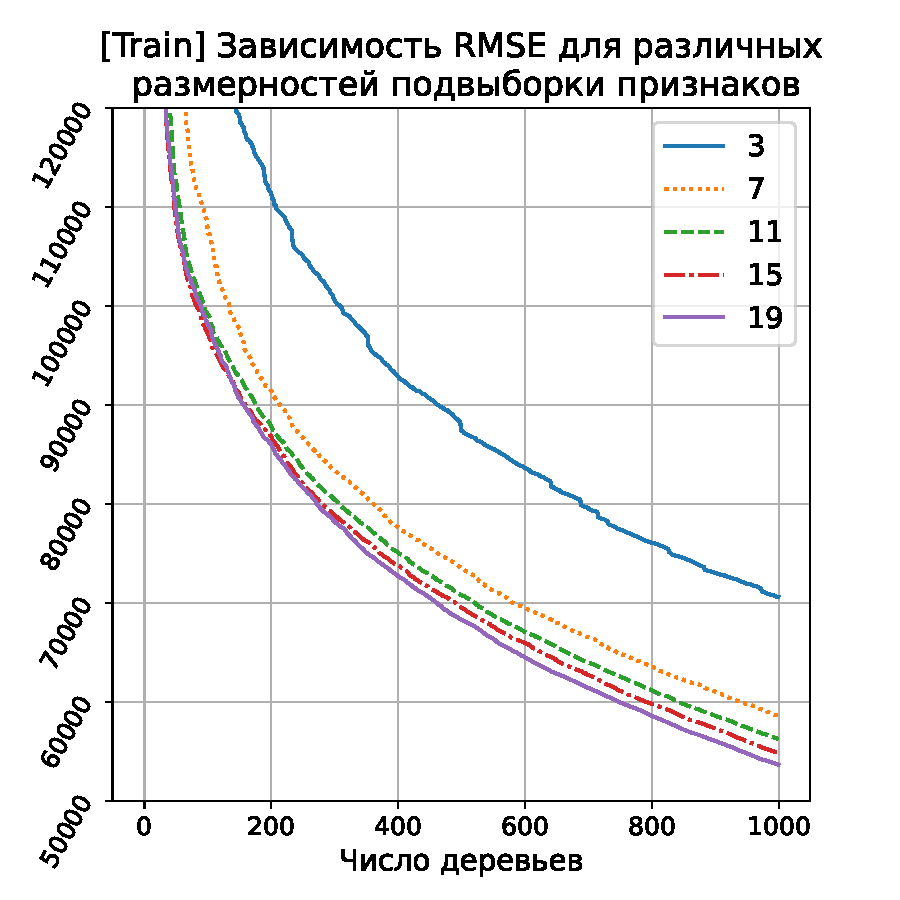
\includegraphics[width=1\linewidth]{3_3.pdf}}
\end{minipage}
\hfill
\begin{minipage}[h]{0.5\linewidth}
\center{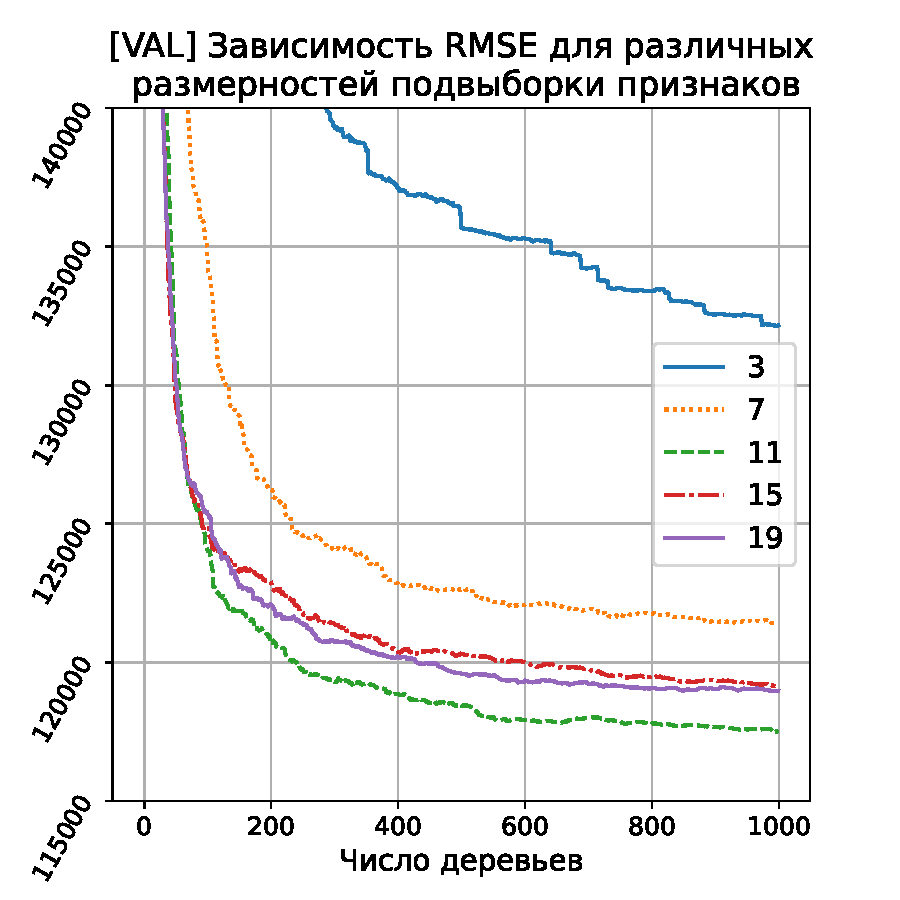
\includegraphics[width=1\linewidth]{3_4.pdf}}
\end{minipage}
\caption{Исследование поведения алгоритма в зависимости от размерности признакового пространства}
\label{ris:image1}
\end{figure}

По графикам зависимости \emph{RMSE} от размерности признакового пространства видно, что на валидационной выборке увеличение количества признаков необязательно влечет уменьшение \emph{RMSE}, как это было в случае с методом случайных лесов, наилучшая точность на валидации достигается на 11 признаках. В случайном лесе данный признак являлся одним из важнейших, что подтверждается графиками выше, при смене данного параметра ошибка изменялась значительно. В градиентном бустинге для размерностей 11, 15 и 19 эта разница не так существенна.


При анализе зависимости максимальной глубины деревьев размерность признакового пространства была выбрана, равной 11, остальные параметры по умолчанию. В градиентном бустинге используются неглубокие деревья, потому что использование глубоких ведет к переобучению. Так, в случае неограниченной глубиной на обучающей выборке была достигнута нулевая ошибка, однако на валидации результат значительно хуже, модель переобучилась. Оптимальным параметром для максимальной глубины является 5. 

\begin{figure}[h!]
\begin{minipage}[h]{0.5\linewidth}
\center{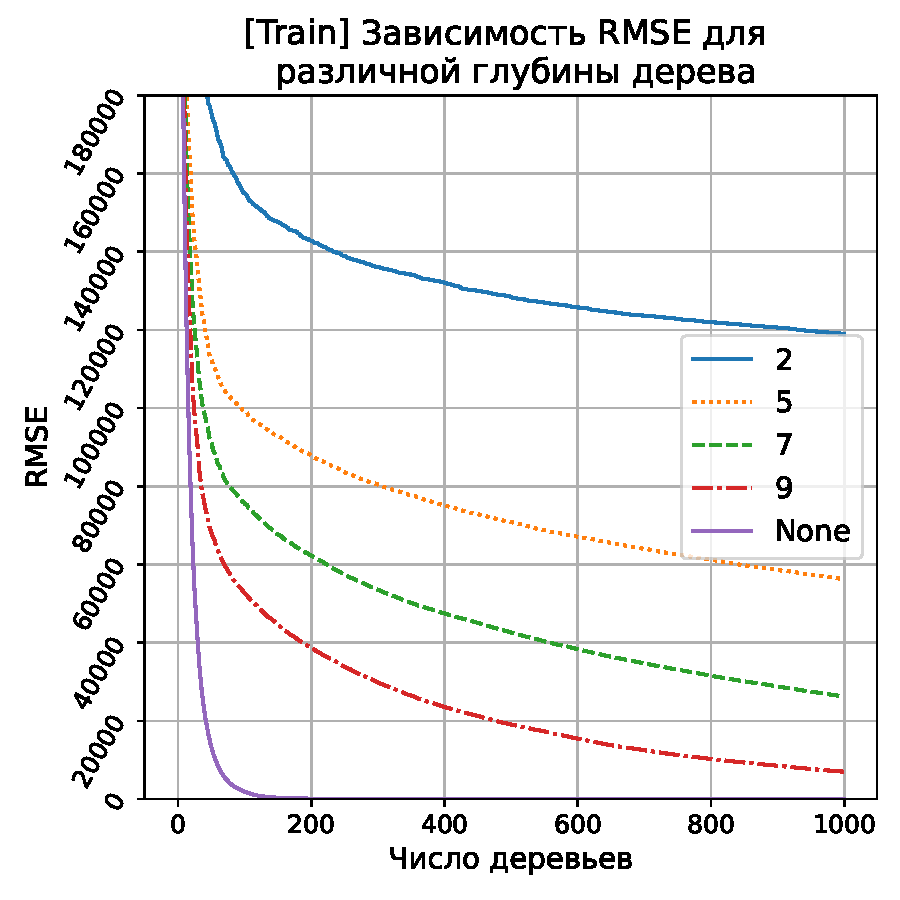
\includegraphics[width=1\linewidth]{3_6.pdf}}
\end{minipage}
\hfill
\begin{minipage}[h]{0.5\linewidth}
\center{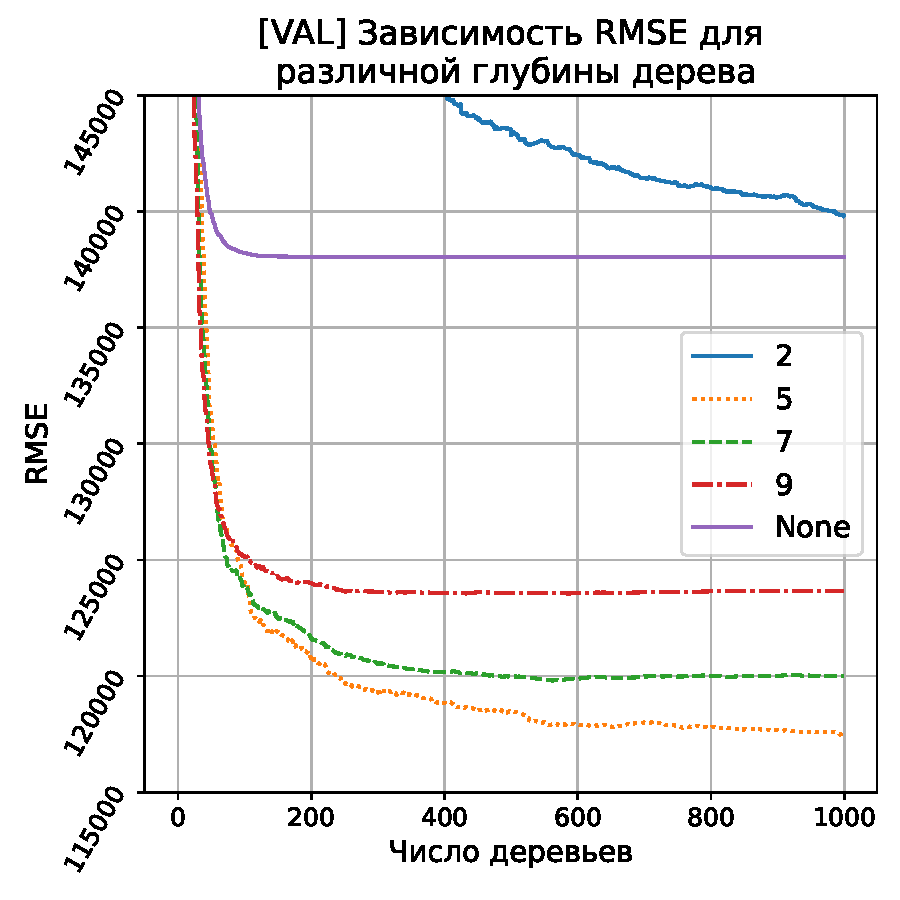
\includegraphics[width=1\linewidth]{3_7.pdf}}
\end{minipage}
\caption{Исследование поведения алгоритма в зависимости от максимальной глубины дерева}
\label{ris:image1}
\end{figure}

\begin{figure}[h!]
\begin{minipage}[h]{0.5\linewidth}
\center{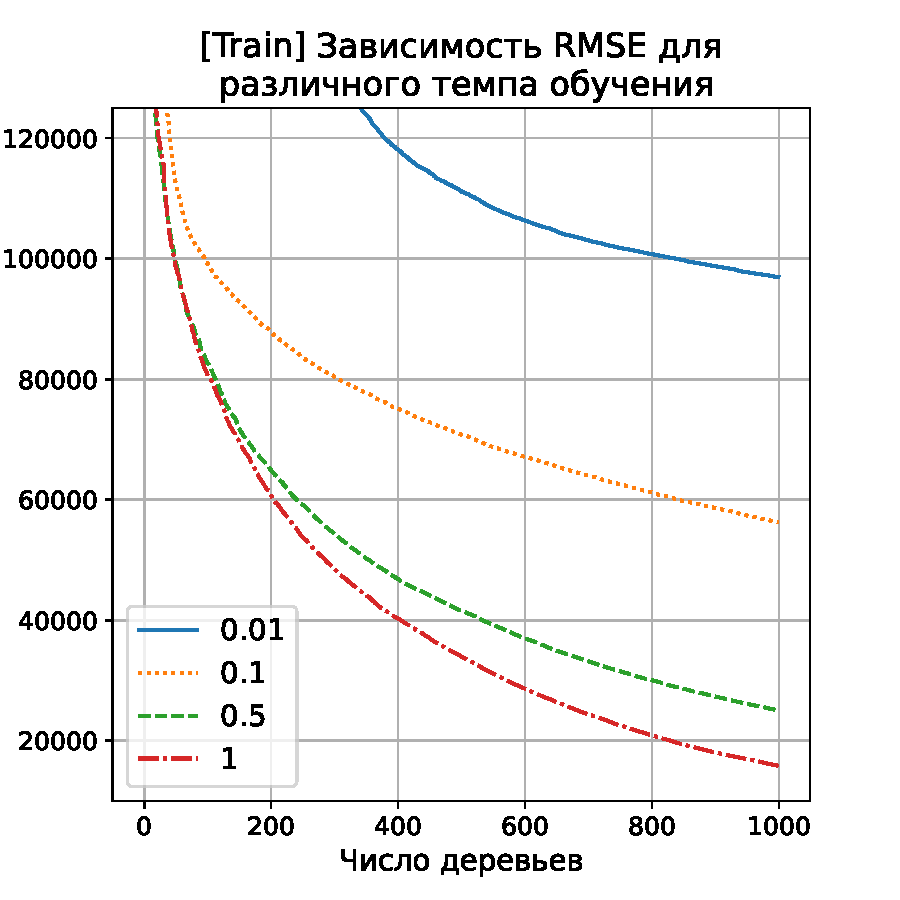
\includegraphics[width=1\linewidth]{3_9.pdf}}
\end{minipage}
\hfill
\begin{minipage}[h]{0.5\linewidth}
\center{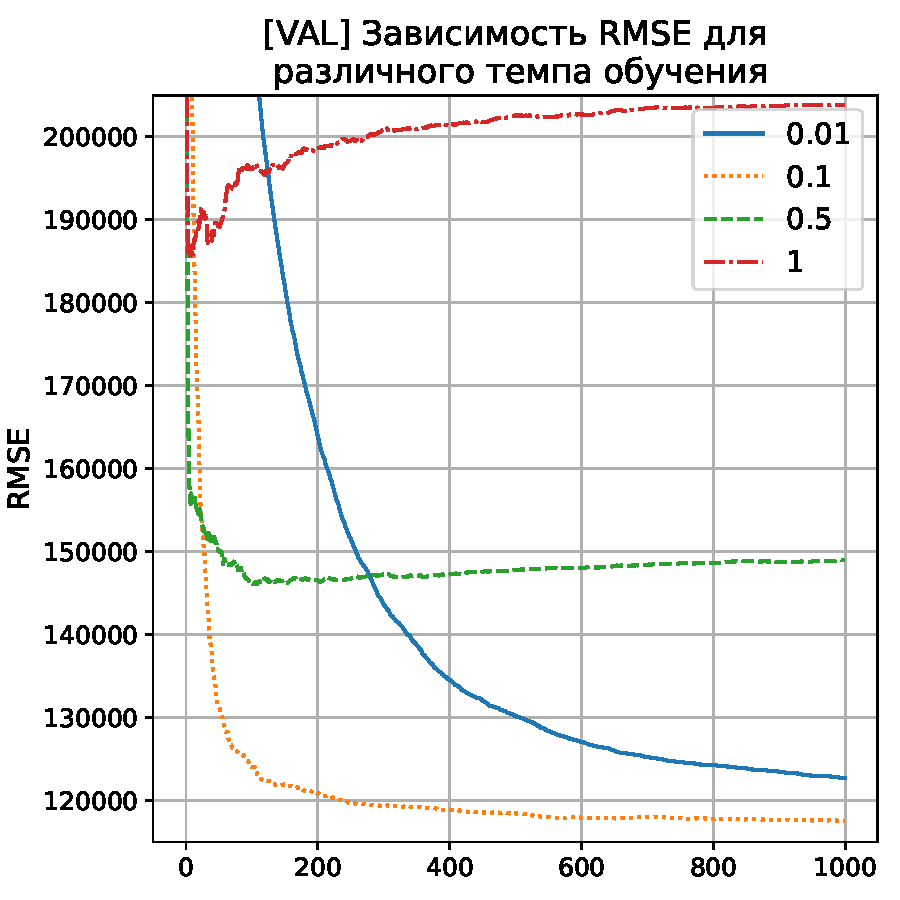
\includegraphics[width=1\linewidth]{3_10.pdf}}
\end{minipage}
\caption{Исследование поведения алгоритма в зависимости от темпа обучения}
\label{ris:image1}
\end{figure}

Анализ поведения алгоритма в зависимости от темпа обучения проводился с фиксированными параметрами: максимальная глубина, равная 5, и размерность пространства признаков, равная 11. На графике зависимости темпа обучения для тренировочной выборки наблюдается, что с ростом темпа обучения ошибка уменьшается, однако на графике для валидации наблюдается переобучение с некоторого момента, монотонная зависимость отсутствует. Оптимальным параметром, отвечающим за темп обучения, является значение 0.1. 

\begin{figure}[h!]
\begin{minipage}[h]{0.5\linewidth}
\center{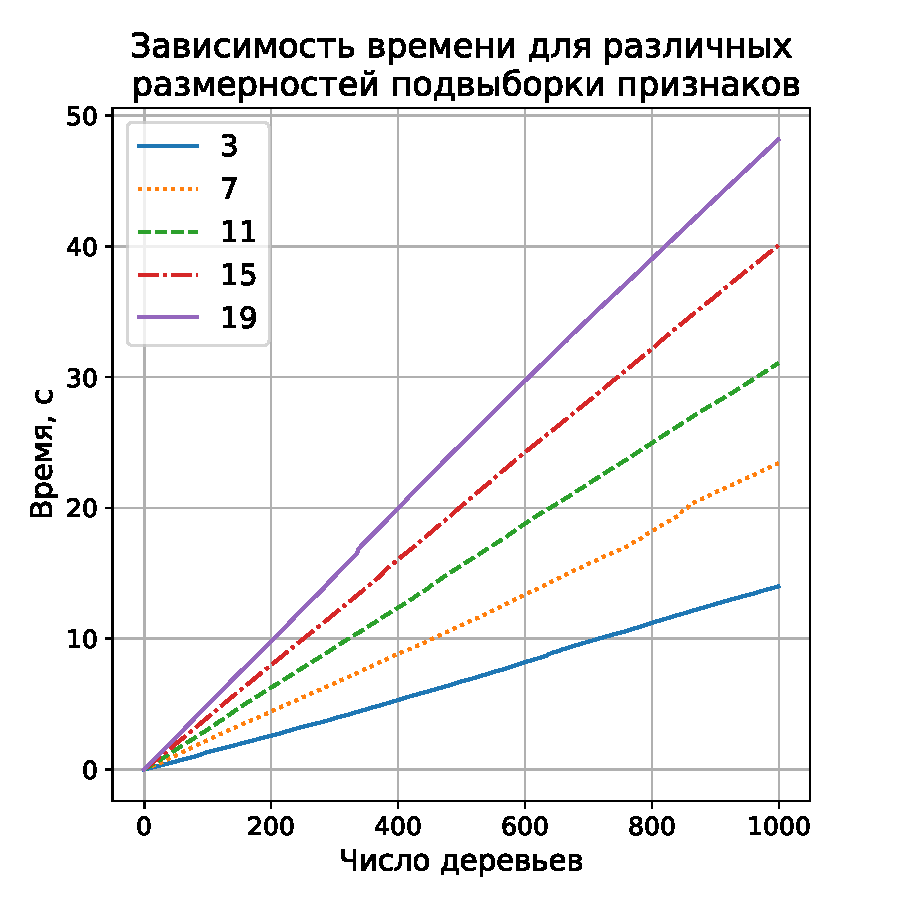
\includegraphics[width=1\linewidth]{3_5.pdf}}
\end{minipage}
\hfill
\begin{minipage}[h]{0.5\linewidth}
\center{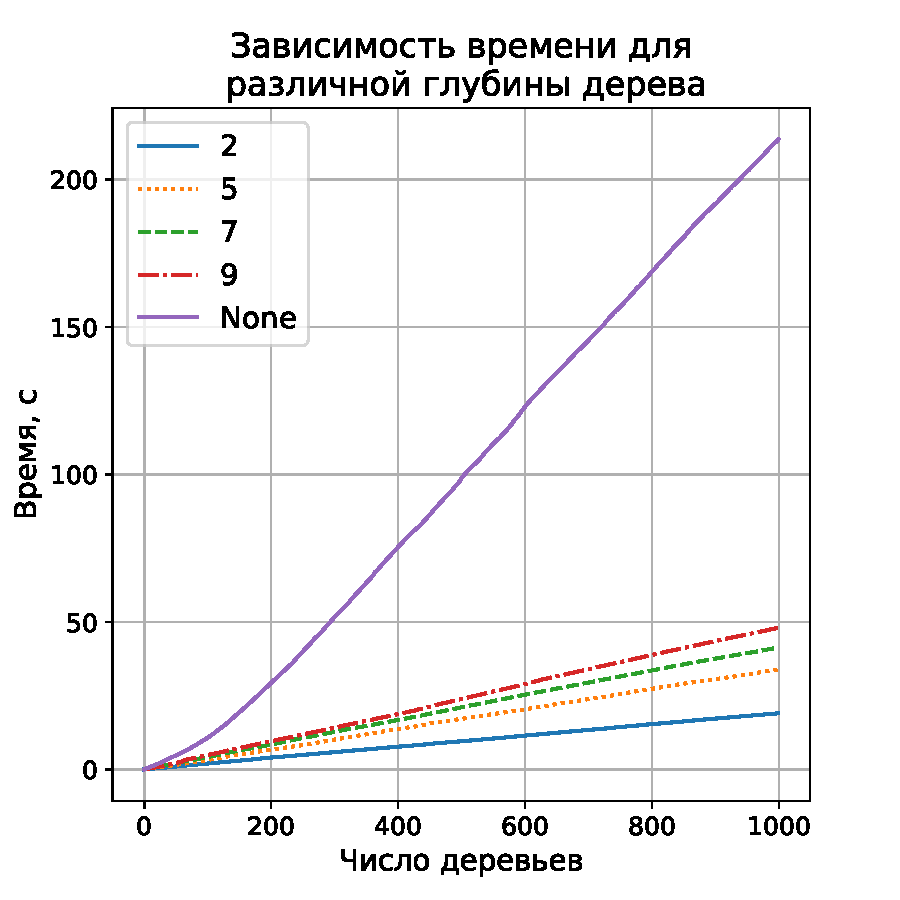
\includegraphics[width=1\linewidth]{3_8.pdf}}
\end{minipage}
\caption{Исследование времени  работы алгоритма в зависимости от параметров}
\label{ris:image1}
\end{figure}

По графику зависимости времени для различных размерностей подвыборки признаков видно, что с ростом числа признаков время работы алгоритма возрастает, что наблюдается и на втором графике зависимости времени от максимальной глубины деревьев. При фиксированном числе деревьев расстояния между прямыми одинаковое, что говорит о линейной зависимости времени от размерности признакового пространства. График зависимости времени от темпа обучения не представляет интереса, так как время работы алгоритмов с различным $learning\_rate$ практически не отличается.
\end{section}

\begin{section}{Общие выводы}
В ходе выполнения задания были изучены два алгоритма композиции решающих деревьев  — случайный лес и градиентный бустинг. В методе случайного леса алгоритмы строятся паралельно, а в случае с градиентным бустингом последововательно, исправляя ошибки предыдущих алгоритмов. В данном задании было проведено исследование поведения алгоритмов при различных параметрах, а также подобраны оптимальные для предоставленных данных. В результате меньшая ошибка с меньшими временными затратами была получена с помощью метода градиентного бустинга.
\end{section}
\end{document}
